%==============================================================================
% CB-SAFE: full paper (IEEEtran conference). Compile:
%   pdflatex cbsafe && pdflatex cbsafe
% References are inline (thebibliography); no bibtex pass required.
% Figures are produced by experiments/plots.py into results/figs/.
%==============================================================================
\documentclass[conference]{IEEEtran}
\IEEEoverridecommandlockouts
\usepackage{cite}
\usepackage{amsmath,amssymb}
\usepackage{booktabs}
\usepackage{graphicx}
\usepackage[T1]{fontenc}
\newtheorem{definition}{Definition}
\newtheorem{theorem}{Theorem}
\newtheorem{proposition}{Proposition}
\graphicspath{{../results/figs/}}

\begin{document}

\title{CB-SAFE: Code-Based Post-Quantum Secure Aggregation\\ for Byzantine-Robust Federated Learning}

\author{
\IEEEauthorblockN{Md Wahiduzzaman Suva (26-94088-2)\qquad Esm-e Moula Chowdhury Abha (26-94089-2)}
\IEEEauthorblockA{Department of Computer Science, American International University-Bangladesh\\
wshuvo360@gmail.com}
}

\maketitle

\begin{abstract}
Secure aggregation protects federated learning (FL) updates by revealing only their
sum, but its key establishment breaks under a quantum adversary, and post-quantum FL
today derives confidentiality almost exclusively from lattice assumptions, a single
point of cryptanalytic failure. We present CB-SAFE, to our knowledge the first FL
secure-aggregation framework whose post-quantum confidentiality is established by a
code-based KEM (HQC, selected by NIST in March 2025 to diversify away from lattices)
rather than a lattice KEM. CB-SAFE treats the KEM as a pluggable module: the same
double-masking protocol runs over HQC or ML-KEM, and per-round mask seeds are derived
from long-lived encapsulated secrets, so the KEM affects only a one-time setup.
Measured on a 291\,498-parameter model with 30 clients, per-round traffic is
KEM-independent (2\,277~KiB per client), and the entire code-based premium is a
one-time 15.2 vs.\ 3.8~KiB per client at NIST level~1 (49.4 vs.\ 7.7~KiB at level~5),
under 0.03\% of the traffic of a single training round. CB-SAFE further reconciles
secure aggregation with Byzantine robustness by aggregating securely \emph{within}
clusters of $c$ clients and applying robust rules (trimmed mean, median, Multi-Krum)
\emph{across} the revealed cluster sums, and we quantify the resulting
privacy--robustness tension: the anonymity set grows with $c$ while the probability a
cluster sum stays uncontaminated decays as $(1-f)^{c}$ under malicious fraction $f$.
We prove a simulation-based privacy theorem, identify a \emph{laundering} effect by
which cluster averaging turns amplified sign-flip poisoning into plausible-magnitude
inverted sums that defeat all coordinate-wise robust rules, and introduce CB-SAFE+:
re-randomized clustering with root-anchored direction flags accumulates per-client
suspicion across rounds (temporal group testing over private sums) and excludes
attackers the server never observes individually, at zero additional leakage.
Experiments across three datasets and two modalities (non-IID CIFAR-10 and
FashionMNIST, and tabular Edge-IIoTset IoT intrusion detection) with
label-flipping, sign-flipping, and backdoor attacks validate the framework: the
laundering effect and CB-SAFE+'s recovery replicate on every dataset (CB-SAFE+
beats every baseline under sign-flip, Holm-corrected $p{<}0.01$), and the
implementation is released open-source.
\end{abstract}

\begin{IEEEkeywords}
Post-quantum cryptography, federated learning, secure aggregation, HQC, code-based
cryptography, Byzantine robustness, cryptographic diversity.
\end{IEEEkeywords}

\section{Introduction}
Federated learning (FL) trains a shared model across many clients without
centralizing data, but the transmitted model updates leak private information:
gradient-inversion and membership-inference attacks reconstruct training samples from
individual updates. Secure aggregation closes this channel by ensuring the server
observes only the \emph{sum} of updates, using pairwise additive masks that cancel on
aggregation \cite{bonawitz2017,bell2020}. The confidentiality of those masks rests on key
establishment that Shor's algorithm breaks once a cryptographically relevant quantum
computer exists, and traffic recorded today can be decrypted then
(``harvest-now, decrypt-later'').

The standard response replaces classical key exchange with a post-quantum KEM, and
nearly all post-quantum FL does so with \emph{lattice} cryptography
\cite{pqsf2024,qinxu2025,narsimhulu2026,nguyen2025lattice,byzpqfl2026}. Lattices are
efficient and standardized (ML-KEM, FIPS~203 \cite{fips203}), but concentrating an
entire ecosystem's confidentiality on one hardness assumption is a systemic risk: a
single cryptanalytic advance would break every such deployment simultaneously. NIST
recognized exactly this risk when, in March~2025, it \emph{selected} the code-based
KEM HQC (whose security reduces to syndrome decoding of quasi-cyclic codes, not to
lattice problems) as a diversified backup to ML-KEM \cite{nistir8545}. That
diversity has not reached federated learning.

A second, orthogonal tension is that secure aggregation and Byzantine robustness pull
in opposite directions: hiding individual updates denies the server exactly the
visibility that poisoning defenses need. Recent work combines robustness with
\emph{lattice}-based post-quantum aggregation \cite{byzpqfl2026}, or achieves
cluster-based robust aggregation on \emph{quantum hardware} \cite{cqsa2026}; no prior
framework provides both under a code-based, classical post-quantum assumption.

This paper presents CB-SAFE (Code-Based Secure Aggregation for Federated
lEarning), making four contributions:
\begin{enumerate}
\item \textbf{A KEM-agnostic secure-aggregation protocol} (Definition~1) that
formalizes Bonawitz-style double masking over any IND-CCA2 KEM, with per-round mask
seeds derived from long-lived encapsulated secrets so key encapsulation is a one-time
cost. The post-quantum primitive becomes a single replaceable module.
\item \textbf{The first code-based instantiation, scope-qualified:} to our knowledge,
CB-SAFE is the first FL secure-aggregation framework whose post-quantum
confidentiality comes from the NIST-selected code-based KEM (HQC) rather than a
lattice KEM, at matched NIST security levels.
\item \textbf{A quantified reconciliation of privacy and robustness:} secure
aggregation \emph{within} clusters of $c$ clients, robust aggregation (trimmed mean,
median, Multi-Krum) \emph{across} cluster sums, and an explicit trade-off law (the
anonymity set is $c$ while the clean-cluster probability decays as $(1-f)^c$)
validated experimentally under three attacks. We further identify and analyze a
\emph{laundering} effect: cluster averaging turns amplified sign-flip poisoning into
plausible-magnitude, direction-inverted cluster sums that defeat every
coordinate-wise robust rule (Proposition~\ref{prop:launder}).
\item \textbf{CB-SAFE+, a defense that identifies hidden attackers:} per-round
re-randomized clustering plus direction flags against a small server root dataset
accumulate per-client suspicion (temporal group testing over privacy-preserving
observations) and exclude malicious clients the server has never observed
individually. The flags are post-processing of already-revealed cluster sums, so the
defense adds \emph{no} leakage beyond CB-SAFE itself (Theorem~\ref{thm:priv}).
\item \textbf{An honest, measured cost analysis:} on a 291k-parameter model,
per-round traffic is KEM-independent and the full code-based premium is a one-time
15.2~KiB vs.\ 3.8~KiB per client (NIST level~1), i.e., under $0.03\%$ of one round's
traffic; HQC's $\sim$200$\times$ slower operations contribute about 2\,s (one-time,
30 clients) versus 0.02\,s for ML-KEM.
\end{enumerate}

\section{Related Work}
\textbf{Post-quantum FL is lattice-dominated.} PQSF reconstructs masks with lattice
multi-stage secret sharing \cite{pqsf2024}; Qin and Xu build single-round aggregation
from a lattice key-homomorphic PRF \cite{qinxu2025}; Narsimhulu \emph{et al.}
aggregate Dilithium-style lattice signatures \cite{narsimhulu2026}; and a 2026
framework combines reputation-weighted Byzantine-robust aggregation with
Kyber/lattice-based secure aggregation for IoT threat intelligence
\cite{byzpqfl2026}. Surveys confirm lattice dominance across post-quantum deployment
\cite{nguyen2025lattice}. Non-lattice exceptions are rare and code-free: multivariate
cryptography with blockchain \cite{singh2025pqfog}, and CQSA, which partitions
clients into clusters aggregated via GHZ states on near-term \emph{quantum hardware}
\cite{cqsa2026}. CB-SAFE differs from all of the above on the confidentiality
assumption: syndrome decoding of quasi-cyclic codes, via a standard-track classical
KEM \cite{nistir8545}, with the KEM exposed behind an agnostic interface so lattice
and code-based variants differ in exactly one module.

\textbf{Cluster-based robust aggregation.} Outside the post-quantum setting,
reconciling Byzantine resilience with secure aggregation is an established goal:
BREA does so through secret-shared distance computation \cite{brea2021}, and CQSA
through clustered aggregation on quantum hardware \cite{cqsa2026}. Aggregating
within groups and inspecting group sums is thus a known structure; our contribution is not the cluster topology itself but (i) its
first classical post-quantum, code-based instantiation and (ii) an explicit,
experimentally validated statement of the privacy--robustness trade-off it induces
(Section~\ref{sec:tradeoff}).

\section{The CB-SAFE Framework}

\begin{figure*}[t]
\centering

\includegraphics[width=\textwidth]{fig_architecture.pdf}
\caption{CB-SAFE, one training round end to end. A one-time code-based (HQC) key
setup establishes pairwise secrets reused every round. In the confidentiality
layer, clients mask updates so masks cancel within clusters of size $c$; the server
observes only the $k$ cluster sums (anonymity set $c$), never an individual update.
The Byzantine-robustness stage (CB-SAFE+) flags clusters by a loss-probe or, in the
trust-free variant, a consensus test; accumulates per-client suspicion across
re-randomized rounds; adaptively excludes identified attackers; and robustly
aggregates the clean cluster sums into the global model, which is broadcast back.}
\label{fig:arch}
\end{figure*}

\subsection{System and Threat Model}
A server coordinates $N$ clients running FedAvg over non-IID data partitions.
Clients are partitioned into $k=N/c$ fixed clusters of size $c$. The server is
honest-but-curious; a fraction $f$ of clients are malicious and submit poisoned
updates; clients may drop out mid-round. Within a cluster, mask recovery uses a
$t$-of-$c$ threshold with $t=\lfloor c/2\rfloor+1$, so privacy holds against the
server colluding with up to $t-1$ members of a cluster, and any $c-t$ members can
drop without stalling the round. Update authentication is out of the code-based
scope: HQC cannot sign and no code-based signature is standardized, so where
signatures are required we compose the lattice-based ML-DSA and state explicitly
that only the confidentiality layer is code-based.

\subsection{KEM-Agnostic Masked Aggregation}
\begin{definition}[KEM-agnostic cluster masking]\label{def:kem}
Let $\mathcal{K}=(\mathrm{KeyGen},\mathrm{Encaps},\mathrm{Decaps})$ be an IND-CCA2
KEM, $H$ a key-derivation function, and $G$ a PRG into $(\mathbb{Z}_{2^{64}})^d$.
At setup, each client $i$ publishes $pk_i$; for each cluster pair $i<j$, client $i$
computes $(ct_{ij}, ss_{ij})=\mathrm{Encaps}(pk_j)$ and $j$ recovers
$ss_{ij}=\mathrm{Decaps}(sk_j, ct_{ij})$. In round $r$, client $i$ quantizes its
update $x_i$ to $q(x_i)\in(\mathbb{Z}_{2^{64}})^d$, draws a self-mask seed $b_i^r$,
Shamir-shares it $t$-of-$c$ within its cluster, and submits
\[
y_i \;=\; q(x_i) + G(b_i^r) + \textstyle\sum_{j>i} G\!\big(H(ss_{ij}, r)\big)
      - \textstyle\sum_{j<i} G\!\big(H(ss_{ij}, r)\big) ,
\]
all mod $2^{64}$, sums over the cluster peers of $i$. The server adds each cluster's
submissions (pairwise masks cancel), reconstructs each survivor's $b_i^r$ from $t$
shares and removes $G(b_i^r)$; for a dropped client $d$, each survivor $j$ reveals
the per-round seed $H(ss_{dj}, r)$ and the server removes the orphaned mask halves.
The server thus obtains exactly $\sum_{i \in \mathrm{alive}} q(x_i)$ per cluster.
\end{definition}

Correctness is exact: masking is modular-arithmetic exact, and the only deviation
from plain float aggregation is fixed-point quantization ($2^{-16}$ per coordinate).
Because encapsulation happens once and per-round seeds come from $H(ss_{ij}, r)$,
per-round messages contain no KEM material at all: the masked update is $8d$ bytes
regardless of the KEM, and the KEM's key and ciphertext sizes appear only in the
one-time setup. Instantiating $\mathcal{K}$ with HQC gives the code-based variant;
with ML-KEM \cite{fips203}, the lattice baseline.

\begin{theorem}[Privacy against honest-but-curious coalitions]\label{thm:priv}
Assume $\mathcal{K}$ is IND-CCA2, $H$ is a secure KDF, and $G$ is a secure PRG. Fix
a cluster $C$ of size $c$ with threshold $t=\lfloor c/2\rfloor+1$, and let the
adversary $\mathcal{A}$ comprise the honest-but-curious server and any $T \subset C$
with $|T| \le t-1$. There exists a PPT simulator that, given only the corrupted
clients' inputs and the sum $\sum_{i \in \mathrm{alive}(C)\setminus T} q(x_i)$,
produces a view computationally indistinguishable from $\mathcal{A}$'s view of a
CB-SAFE round. The CB-SAFE+ flag bits are a deterministic function of the revealed
cluster sums and server-local data, so CB-SAFE+ leaks nothing beyond CB-SAFE.
\end{theorem}

\emph{Proof sketch.} A hybrid argument. (H1) Replace each pairwise secret $ss_{ij}$
between honest clients by a uniform string: distinguishing H1 from the real game
breaks IND-CCA2 of $\mathcal{K}$. (H2) Replace the per-round seeds $H(ss_{ij},r)$
and mask streams $G(\cdot)$ by uniform: breaks the KDF/PRG. In H2 every honest
submission $y_i$ is uniform subject to the alive-honest submissions summing to the
revealed cluster sum, which the simulator can sample directly. Shamir shares held by
$\le t-1$ corrupted parties are uniform by perfect secrecy below the threshold, and
a dropped client's revealed seeds $H(ss_{dj}, r)$ are independent of other rounds'
seeds under the KDF assumption, so both recovery paths are simulatable. Distinct
rounds use distinct seeds, so views compose across rounds. \hfill$\square$

The anonymity set of an honest client is therefore its cluster's alive honest-member
count, and re-randomizing the partition each round (CB-SAFE+) does not change the
per-round argument because each round reveals sums of fresh, independently masked
updates.

\subsection{Robust Aggregation Across Cluster Sums}\label{sec:tradeoff}
The server sees $k$ cluster sums $S_1,\dots,S_k$ (means after dividing by alive
counts) and no individual update. CB-SAFE applies a robust rule across the cluster
means: coordinate-wise trimmed mean (trim $\beta$ per side) or median \cite{yin2018},
or Multi-Krum \cite{blanchard2017}. This resolves the hide-versus-inspect tension structurally (privacy
is enforced below the cluster boundary, robustness operates above it) at a
quantifiable price. A cluster mean is contaminated if it contains at least one
malicious member, so with malicious fraction $f$ and random cluster assignment,
\[
\Pr[\text{cluster clean}] = (1-f)^{c},
\]
and the expected number of clean cluster means is $k(1-f)^c$. Larger $c$ improves
privacy (bigger anonymity set) but shrinks the clean fraction the robust rule can
rely on; a trimmed mean discarding $\beta$ per side tolerates at most
$\lfloor \beta k \rfloor$ contaminated clusters. $c$ is therefore a tunable
privacy--robustness dial, and Section~\ref{sec:eval} traces its consequences
empirically. Setting $c{=}1$ recovers classical (privacy-free) robust aggregation;
setting $c{=}N$ recovers full secure aggregation with no robustness.

The contamination probability, however, understates the problem: cluster averaging
also \emph{disguises} what it contaminates.

\begin{proposition}[Laundering by cluster averaging]\label{prop:launder}
Let each honest update be $h$ (up to noise) and let $m$ members of a cluster of size
$c$ submit the scaled sign-flip $-\gamma h$. The cluster mean is
$\mu = \frac{c - m(1+\gamma)}{c}\, h$. Its magnitude equals an honest cluster's
($|\mu| = |h|$) exactly when $\gamma = 2c/m - 1$, while its direction is inverted.
At the common attack setting $\gamma{=}5$ with $c{=}3$, $m{=}1$ this holds with
equality: the poisoned cluster sum is indistinguishable from honest by any
magnitude- or order-statistic test, and a near-symmetric $\pm h$ population drives
coordinate-wise trimmed mean and median toward $0$, stalling learning entirely.
\end{proposition}

This laundering effect explains the empirical collapse of every coordinate-wise
rule in Section~\ref{sec:eval} and motivates direction-based detection: what
cluster averaging cannot hide is the \emph{sign} of the update.

\subsection{CB-SAFE+: Temporal Group Testing over Cluster Sums}\label{sec:defense}
CB-SAFE+ turns the laundering signature into an identification mechanism, using
three ingredients. (i)~\emph{Re-randomized clustering}: the partition is redrawn
every round (pairwise secrets with all peers are established once at setup, so
re-clustering adds no per-round KEM cost). (ii)~\emph{Loss-probe flags}: the
server maintains a small root dataset ($|D_0|{=}200$ samples held out from all
clients, the standard trust-bootstrapping assumption \cite{fltrust,zeno}), applies
each cluster mean to the current model, and flags every cluster whose mean
\emph{increases} root loss. Flags are computed from already-revealed cluster sums
and server-local data, so they add no leakage (Theorem~\ref{thm:priv}). The probe is
the product of two measured failures. Anchor-free direction flags are
sign-ambiguous: the poisoned cluster sums form their own coherent cloud at $-h$, and
a Krum-based reference locks onto that cloud in a large fraction of rounds.
Anchored \emph{cosine} flags break the symmetry but lose specificity under non-IID
data: an $m{=}1$ poisoned cluster mean is dominated by $-\gamma$ times one client's
idiosyncratic direction, nearly orthogonal to the balanced anchor, so its sign test
approaches a coin flip (at $f{=}0.2$ we measured cosine flags hitting clean clusters
as often as dirty ones, and suspicion never separated). The loss probe is immune to
this decorrelation because a $\gamma$-amplified ascent direction raises root loss
regardless of whose data dominates the cluster sum. (iii)~\emph{Suspicion accumulation and exclusion}: every member of a flagged
cluster gains one suspicion count. A malicious client sits in a flagged cluster in
essentially every round, while an honest client is flagged only when randomly
co-clustered with an attacker, i.e., with probability $p_h = 1-(1-f)^{c-1} < 1$.
After $R$ rounds the flagged fractions separate (by Hoeffding, misclassification
probability decays as $e^{-2R(\tau - p_h)^2}$ for a threshold $\tau$ between $p_h$
and $1$), and clients whose fraction exceeds $\tau$ ($0.85$ here, after a 5-round
warmup) are excluded. The server thereby identifies individual attackers it has
never observed individually: group testing where the pools are the
privacy-preserving cluster sums and the tests repeat over training rounds.

\section{Implementation}
CB-SAFE is implemented in Python on liboqs~0.15.0 (via \texttt{liboqs-python}) and
PyTorch, with the KEM selected by a one-line configuration change among HQC-128/192/256
and ML-KEM-512/768/1024 (Kyber round-3 parameter sets are retained for comparison
with older literature). Masks are ChaCha20 keystreams; per-round seeds use
HKDF-SHA256; self-mask seeds are shared with Shamir's scheme over
$\mathrm{GF}(2^{127}-1)$. \emph{HQC provenance:} liboqs~0.15.0 ships the PQClean
constant-time implementation of the Round-4 HQC specification (2023-04-30), the
version NIST evaluated and selected \cite{nistir8545}; the finalized standard's
parameters may differ slightly once published (a draft is expected as FIPS~207).
Federated training is simulated in-process; every protocol byte count and crypto
timing reported below is measured from real objects on the wire path of the
protocol (public keys, ciphertexts, shares, masked vectors), not modeled.
\emph{Reproducibility:} Python 3.12, PyTorch 2.5.0 (CUDA 12.4), liboqs-python
0.15.0, on a single NVIDIA RTX 2060 (6\,GB); one training round of 30 clients takes
$\approx$21\,s. All runs use fixed seed 0 with deterministic partitioning and
cluster assignment; CIFAR-10 and FashionMNIST results are averaged over three seeds
(Edge-IIoTset over one), significance is by paired $t$-test with Holm correction,
and every experiment is reproducible from a per-run CSV and the released scripts.

\section{Evaluation}\label{sec:eval}
\subsection{Setup}
\textbf{Task and data.} Primary task: CIFAR-10 partitioned across $N{=}30$ clients
by a Dirichlet($\alpha{=}0.5$) label-skew split; a CNN with $d{=}291\,498$
parameters; one local epoch per round (SGD, lr $0.01$, momentum $0.9$, batch $64$);
$k{=}10$ clusters of $c{=}3$ unless stated. Generalization (Section~\ref{sec:general})
adds FashionMNIST (same CNN) and Edge-IIoTset (a 15-class tabular IoT
intrusion-detection set with a multilayer perceptron), each Dirichlet-partitioned
identically. \textbf{Configurations.} Plain FedAvg (no
cryptography); CB-SAFE/lattice (ML-KEM); CB-SAFE/code-based (HQC), at matched NIST
levels. \textbf{Attacks.} Label flipping ($y \to 9-y$), sign flipping
($-5\Delta$), and a backdoor \cite{bagdasaryan2020} (3$\times$3 trigger patch,
target class~0, 50\% local poison rate) at malicious fractions $f \in \{0.1, 0.2, 0.3\}$, against aggregation
rules mean, trimmed mean, median, Multi-Krum, and the CB-SAFE+ reputation defense
(Section~\ref{sec:defense}; server root set of 200 samples held out from all
clients). \textbf{Metrics.} Test accuracy;
backdoor attack success rate (ASR: fraction of triggered non-target test samples
classified as the target); communication bytes per client (setup vs.\ per-round);
crypto wall-time; dropout-recovery cost.

\subsection{Overhead: the Code-Based Premium Is a One-Time Cost}
Table~\ref{tab:overhead} reports measured per-client traffic and crypto time.
Per-round traffic is identical across all six KEMs (2\,277~KiB per client,
dominated by the $8d$-byte masked update plus 102~B of Shamir material) because
Definition~\ref{def:kem} keeps KEM objects out of the per-round path entirely. The
KEM appears only in setup: at NIST level~1, HQC costs 15.2~KiB per client against
ML-KEM's 3.8~KiB ($4.0\times$; $6.4\times$ at level~5), and 2.0\,s of one-time
compute for all 30 clients against 0.02\,s. Amortized over 40 training rounds
($\sim$89\,MiB of per-client update traffic), the code-based premium is below
$0.03\%$ of total communication (Fig.~\ref{fig:amort}). A round with 10\% dropouts
adds only seed-reveal messages (32~B per survivor--dropout pair) and kept server
unmasking below 0.28\,s in all configurations. The practicality question that
motivated this work has a quantitative answer: \emph{cryptographic diversity in FL
secure aggregation is essentially free at the protocol level once key establishment
is amortized}: the trade-off is a one-time setup constant, not a per-round tax.

\begin{table}[t]
\caption{Measured per-client overhead ($N{=}30$, $c{=}3$, $d{=}291\,498$).
Setup is one-time; per-round traffic is KEM-independent.}
\label{tab:overhead}
\centering
\footnotesize
\setlength{\tabcolsep}{3.5pt}
\begin{tabular}{@{}lrrrr@{}}
\toprule
KEM & Setup (KiB) & Setup wall (s) & Round (KiB) & Mask (ms) \\
\midrule
ML-KEM-512  & 3.8  & 0.02 & 2\,277 & 25 \\
HQC-128     & 15.2 & 2.0  & 2\,277 & 26 \\
ML-KEM-768  & 5.6  & 0.02 & 2\,277 & 27 \\
HQC-192     & 30.8 & 5.7  & 2\,277 & 25 \\
ML-KEM-1024 & 7.7  & 0.02 & 2\,277 & 25 \\
HQC-256     & 49.4 & 10.6 & 2\,277 & 26 \\
\bottomrule
\end{tabular}
\end{table}

\begin{figure}[t]
\centering
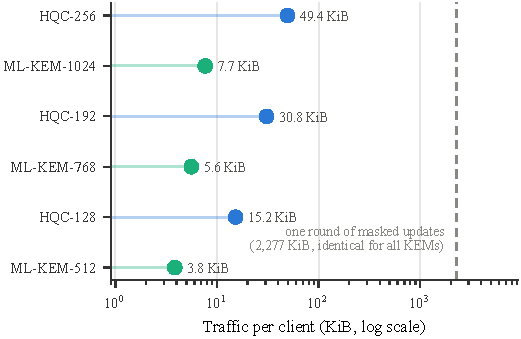
\includegraphics[width=\columnwidth]{fig_amortization.pdf}
\caption{One-time setup traffic per client versus a single round of masked updates
(log scale). Even HQC-256's setup is $\sim$2\% of one round's traffic; per-round
traffic is identical for all KEMs.}
\label{fig:amort}
\end{figure}

\subsection{Utility and Cryptographic Equivalence}
Plain FedAvg reaches 59.0\% test accuracy (mean of the final five of 40 rounds;
59.6\% at round 40) on the non-IID split (Fig.~\ref{fig:utility}). In every round,
the same client updates were pushed through the full cryptographic pipeline twice
(once under HQC-128, once under ML-KEM-768), and every per-cluster secure sum was
compared coordinate-wise against the plain sum. The maximum deviation across all 40
rounds and both KEMs was $2.28\times10^{-5}$, which \emph{equals} the worst-case
fixed-point rounding bound for a 3-element sum ($3\cdot 2^{-17}=2.29\times10^{-5}$):
the masking arithmetic itself is exact, so CB-SAFE's accuracy curve is identical to
plain FedAvg by construction, not approximately. Both dropout modes were exercised:
in round 10, two of three dropped clients landed in the same cluster, driving it
below its $t{=}2$ threshold: the protocol excluded that cluster and recovered the
remaining nine exactly; in round 20, three dropouts in three distinct clusters were
all recovered by seed-reveal plus Shamir reconstruction. Measured in-run, setup cost
2.6\,s (HQC-128) vs.\ 0.02\,s (ML-KEM-768) for all 30 clients, and steady-state
rounds took $\sim$30\,ms of client-side masking and $\sim$0.29\,s of server-side
unmasking, negligible against the $\sim$21\,s of local training per round.

\begin{figure}[t]
\centering
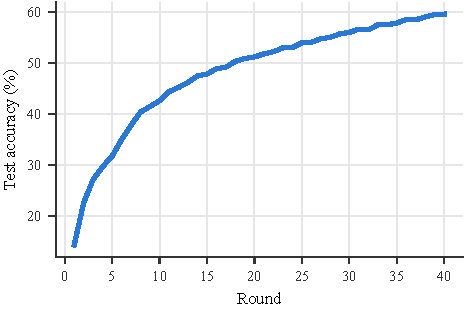
\includegraphics[width=\columnwidth]{fig_utility.pdf}
\caption{Test accuracy of FedAvg on non-IID CIFAR-10; CB-SAFE's secure aggregates
(HQC and ML-KEM) are numerically equivalent to plain aggregation, so the accuracy
curve is shared by all three configurations.}
\label{fig:utility}
\end{figure}

\subsection{Robustness Under Attack}
\textbf{The contamination law holds.} Across all runs, the realized fraction of
clean cluster sums tracked $(1-f)^c$ closely: at $c{=}3$, observed $0.70/0.50/0.40$
versus predicted $0.73/0.51/0.34$ for $f{=}0.1/0.2/0.3$.

\begin{table}[t]
\caption{Robustness of aggregation rules over cluster sums ($c{=}3$, $k{=}10$,
seed 0): final test accuracy under sign-flip and attack success rate (ASR, lower is
better) under the backdoor, at malicious fraction $f$. Best per column in bold.
CB-SAFE+ additionally reports zero honest false-positive exclusions in every
configuration.}
\label{tab:robust}
\centering
\footnotesize
\setlength{\tabcolsep}{3.2pt}
\begin{tabular}{@{}lrrrrrr@{}}
\toprule
& \multicolumn{3}{c}{Sign-flip acc.\ (\%)} & \multicolumn{3}{c}{Backdoor ASR (\%)}\\
\cmidrule(lr){2-4}\cmidrule(l){5-7}
Rule & $f{=}.1$ & $f{=}.2$ & $f{=}.3$ & $f{=}.1$ & $f{=}.2$ & $f{=}.3$\\
\midrule
Mean          & 29.6 & 10.0 & 10.0 & 87.3 & 94.4 & 96.7\\
Trimmed mean  & 42.0 & 10.0 & 10.0 & 79.7 & 93.5 & 96.3\\
Median        & 43.4 & 10.0 & 10.0 & \textbf{40.4} & 93.3 & 96.3\\
Multi-Krum    & \textbf{52.9} & \textbf{42.7} & 16.9 & 86.4 & \textbf{92.4} & 97.2\\
CB-SAFE+      & 51.7 & 37.6 & \textbf{42.8} & -- & 94.2 & \textbf{95.1}\\
\bottomrule
\end{tabular}
\end{table}

\textbf{Sign-flip: laundering collapses coordinate-wise rules exactly at the
predicted boundary} (Table~\ref{tab:robust}, Fig.~\ref{fig:signflip}). At $f{=}0.1$ ($\approx$3 dirty
clusters, within trim capacity) the static rules work: trimmed mean 42.0\%, median
43.4\%, Multi-Krum 52.9\%, versus 29.6\% for the undefended mean and 59\% clean
baseline. At $f{=}0.2$ ($\approx$5 dirty clusters) every coordinate-wise rule is
pinned at exactly 10.0\% (random guessing), not because the model diverges but
because the laundered $\pm h$ population drives the aggregate to zero
(Proposition~\ref{prop:launder}), while Multi-Krum, which selects whole vectors
rather than per-coordinate statistics, still reaches 42.7\% (16.9\% at $f{=}0.3$).
Robust rules that rely on magnitude order statistics are structurally weakened by
the very mechanism that provides privacy; vector-selection rules retain power.

\textbf{CB-SAFE+ restores learning past the static breakdown}
(Table~\ref{tab:robust}). With loss-probe
flags and temporal suspicion, the defense identified all 3 of 3 attackers at
$f{=}0.1$ (51.7\%, near the clean ceiling) and 8 of 9 sign-flip attackers
with \emph{zero} honest false positives at $f{=}0.3$, recovering to 42.8\%
accuracy where every static coordinate-wise rule sat at 10\% and Multi-Krum at
16.9\%, comparable to the 39--41\% the median achieves \emph{without any privacy}
($c{=}1$), i.e., the defense refunds the privacy dial's cost in rounds rather than
anonymity. At $f{=}0.2$ per-round flag filtering alone recovers 37.6\% (exclusions
are rare because $m{=}1$ laundered sums raise root loss only mildly); Multi-Krum's
44\% remains stronger in this moderate regime, so the defense's advantage grows
with attack severity and the two are complementary rather than ranked.
Under label flipping (a weak attack in this regime: all rules land within
44--52\%) the probe flags only the worst clusters and excludes conservatively (zero
false positives at $f{=}0.2$), matching the best static rule.

\textbf{Backdoor: a mechanism-independent blind spot.} The trigger attack leaves
main-task accuracy intact for every rule (50--55\%) while ASR stays at 86--97\%
across mean, trimmed mean, Multi-Krum, \emph{and} CB-SAFE+
(Fig.~\ref{fig:backdoor}): backdoored cluster sums \emph{reduce} clean root loss
and align with the honest direction, so they are invisible to loss- and
direction-based tests alike. The one partial exception is the coordinate-wise
median at $f{=}0.1$, which suppresses ASR to 40\%: order statistics can filter the
trigger direction's coordinates when contamination is sparse. We therefore claim
CB-SAFE+ for \emph{untargeted} model poisoning only; targeted trigger attacks under
secure aggregation remain open, consistent with their difficulty even without
privacy constraints.

\begin{figure}[t]
\centering
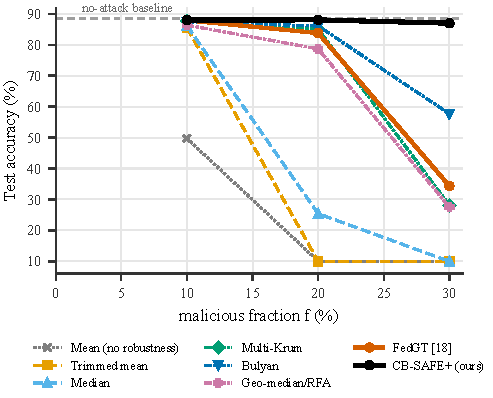
\includegraphics[width=\columnwidth]{fig_signflip_acc.pdf}
\caption{Sign-flip attack ($\gamma{=}5$): accuracy vs.\ malicious fraction across
aggregation rules over $k{=}10$ cluster sums ($c{=}3$). Coordinate-wise rules
collapse at the contamination boundary the $(1-f)^c$ law predicts; vector selection
degrades gracefully; CB-SAFE+ identifies and excludes the attackers.}
\label{fig:signflip}
\end{figure}

\begin{figure}[t]
\centering
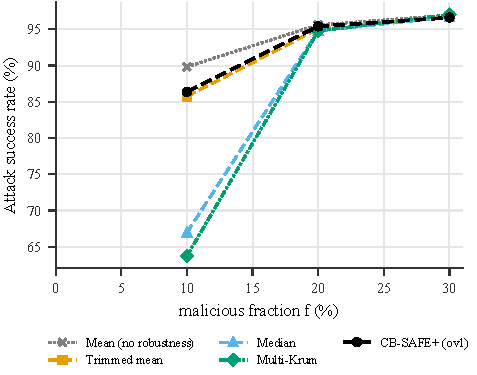
\includegraphics[width=\columnwidth]{fig_backdoor_asr.pdf}
\caption{Backdoor attack success rate vs.\ malicious fraction. No sum-level rule
suppresses the trigger (median at $f{=}0.1$ partially excepted): backdoored sums
help the main task and evade loss/direction probes, the honest scope limit of
robustness under secure aggregation.}
\label{fig:backdoor}
\end{figure}

\subsection{Generalization Across Datasets and Modalities}\label{sec:general}
To test whether the laundering effect and CB-SAFE+'s recovery are artifacts of one
dataset, we repeat the sign-flip evaluation on FashionMNIST (a second image
benchmark, three seeds) and on Edge-IIoTset (tabular IoT/IIoT intrusion detection
with a multilayer perceptron, a different modality in the security domain of the
closest prior work \cite{byzpqfl2026}). The pattern is identical everywhere
(Table~\ref{tab:signflip}, Fig.~\ref{fig:general}): every coordinate-wise rule
collapses to chance at $f{\ge}0.2$ (10.0\% on the 10-class image sets, 7.3\% on
15-class Edge-IIoTset), Multi-Krum degrades gracefully then falls at $f{=}0.3$, and
CB-SAFE+ tracks the clean baseline. At $f{=}0.3$ CB-SAFE+ retains 84\%, high-$80$s,
and 97\% of the no-attack accuracy on CIFAR-10, FashionMNIST, and Edge-IIoTset
respectively, versus 12--18\% for the worst static rule. Pooling all matched
(dataset, $f$, seed) cells, CB-SAFE+ beats every baseline under a paired $t$-test
with Holm correction: versus the mean by 48.3 points ($p{<}10^{-4}$), the median by
37.7 ($p{=}3{\times}10^{-4}$), and Multi-Krum by 11.9 ($p{=}9{\times}10^{-3}$). The
Edge-IIoTset result is the sharpest: at $f{=}0.3$ CB-SAFE+ holds 61.5\% against a
63.7\% clean baseline while mean, trimmed mean, and median all sit at 7.3\%.

\begin{table*}[t]\centering\footnotesize
\caption{Test accuracy (\%) under the sign-flip (laundering) attack across four datasets and malicious fractions $f$ (mean\,$\pm$\,std over 3 seeds for CIFAR-10/FashionMNIST/Edge-IIoTset; single seed for EMNIST). Higher is better; best per column in bold. A dash ($-$) marks a cell still being computed.}
\label{tab:signflip}
\setlength{\tabcolsep}{4pt}
\begin{tabular}{@{}lcccccccccccc@{}}\toprule
& \multicolumn{3}{c}{CIFAR-10} & \multicolumn{3}{c}{FashionMNIST} & \multicolumn{3}{c}{EMNIST} & \multicolumn{3}{c}{Edge-IIoTset}\\
\cmidrule(lr){2-4}\cmidrule(lr){5-7}\cmidrule(lr){8-10}\cmidrule(l){11-13}
Method & $f{=}.1$ & $f{=}.2$ & $f{=}.3$ & $f{=}.1$ & $f{=}.2$ & $f{=}.3$ & $f{=}.1$ & $f{=}.2$ & $f{=}.3$ & $f{=}.1$ & $f{=}.2$ & $f{=}.3$\\\midrule
FedAvg (mean) & 21.4\,{\scriptsize$\pm$8.3} & 10.0\,{\scriptsize$\pm$0.0} & 10.0\,{\scriptsize$\pm$0.0} & 48.9\,{\scriptsize$\pm$28.5} & 10.0\,{\scriptsize$\pm$0.0} & 10.0\,{\scriptsize$\pm$0.0} & \textbf{35.9} & $-$ & $-$ & 43.0\,{\scriptsize$\pm$12.1} & 7.4\,{\scriptsize$\pm$0.2} & 7.4\,{\scriptsize$\pm$0.2}\\
Trimmed mean & 45.4\,{\scriptsize$\pm$2.4} & 10.0\,{\scriptsize$\pm$0.0} & 10.0\,{\scriptsize$\pm$0.0} & 82.7\,{\scriptsize$\pm$1.4} & 10.0\,{\scriptsize$\pm$0.0} & 10.0\,{\scriptsize$\pm$0.0} & $-$ & $-$ & $-$ & 60.2\,{\scriptsize$\pm$1.6} & 8.1\,{\scriptsize$\pm$0.8} & 7.4\,{\scriptsize$\pm$0.2}\\
Median & 47.8\,{\scriptsize$\pm$3.2} & 10.0\,{\scriptsize$\pm$0.0} & 10.0\,{\scriptsize$\pm$0.0} & 83.6\,{\scriptsize$\pm$1.1} & 10.0\,{\scriptsize$\pm$0.0} & 10.0\,{\scriptsize$\pm$0.0} & $-$ & $-$ & $-$ & 60.7\,{\scriptsize$\pm$0.8} & 13.8\,{\scriptsize$\pm$5.1} & 7.4\,{\scriptsize$\pm$0.2}\\
Multi-Krum & 53.6\,{\scriptsize$\pm$0.8} & 39.8\,{\scriptsize$\pm$2.2} & 20.3\,{\scriptsize$\pm$10.1} & 85.9\,{\scriptsize$\pm$0.8} & 83.0\,{\scriptsize$\pm$1.6} & 43.1\,{\scriptsize$\pm$23.9} & $-$ & $-$ & $-$ & 63.2\,{\scriptsize$\pm$0.5} & 57.6\,{\scriptsize$\pm$2.8} & 32.7\,{\scriptsize$\pm$18.6}\\
Bulyan & 53.3\,{\scriptsize$\pm$0.3} & 49.8\,{\scriptsize$\pm$0.9} & 30.8\,{\scriptsize$\pm$16.3} & $-$ & $-$ & $-$ & $-$ & $-$ & $-$ & 62.3\,{\scriptsize$\pm$0.9} & 60.8\,{\scriptsize$\pm$0.5} & 26.1\,{\scriptsize$\pm$25.6}\\
Geo-median / RFA & 46.7 & 36.8 & 10.0 & $-$ & $-$ & $-$ & $-$ & $-$ & $-$ & 61.5\,{\scriptsize$\pm$1.1} & 53.2\,{\scriptsize$\pm$9.2} & 20.9\,{\scriptsize$\pm$18.9}\\
FLTrust & $-$ & 20.6 & 13.2 & $-$ & $-$ & $-$ & $-$ & $-$ & $-$ & 42.0\,{\scriptsize$\pm$1.3} & 35.1\,{\scriptsize$\pm$10.1} & 28.9\,{\scriptsize$\pm$0.5}\\
FedGT [TIFS'25] & \textbf{54.0\,{\scriptsize$\pm$0.2}} & \textbf{51.3\,{\scriptsize$\pm$1.4}} & \textbf{50.1\,{\scriptsize$\pm$1.2}} & 85.8\,{\scriptsize$\pm$0.4} & 86.0\,{\scriptsize$\pm$0.4} & 83.0\,{\scriptsize$\pm$1.6} & $-$ & $-$ & $-$ & 62.8\,{\scriptsize$\pm$0.6} & 62.2\,{\scriptsize$\pm$1.3} & 62.7\,{\scriptsize$\pm$1.0}\\
CB-SAFE+ (ours) & 53.0\,{\scriptsize$\pm$0.6} & 47.1\,{\scriptsize$\pm$2.6} & 37.9\,{\scriptsize$\pm$12.6} & 85.7\,{\scriptsize$\pm$0.5} & 86.0\,{\scriptsize$\pm$0.5} & 83.1\,{\scriptsize$\pm$1.9} & $-$ & $-$ & $-$ & 62.6\,{\scriptsize$\pm$0.5} & 62.5\,{\scriptsize$\pm$0.6} & 62.1\,{\scriptsize$\pm$0.9}\\
CB-SAFE+ ov4 (ours) & 53.5\,{\scriptsize$\pm$0.6} & 49.3\,{\scriptsize$\pm$3.0} & 48.8\,{\scriptsize$\pm$2.0} & \textbf{86.1\,{\scriptsize$\pm$0.4}} & \textbf{86.2\,{\scriptsize$\pm$0.4}} & 84.8\,{\scriptsize$\pm$1.1} & $-$ & $-$ & $-$ & 63.7\,{\scriptsize$\pm$0.6} & 62.9\,{\scriptsize$\pm$0.6} & \textbf{62.7\,{\scriptsize$\pm$0.9}}\\
CB-SAFE+ trust-free (ours) & 54.0\,{\scriptsize$\pm$0.1} & 10.0\,{\scriptsize$\pm$0.0} & 10.0\,{\scriptsize$\pm$0.0} & 85.9\,{\scriptsize$\pm$0.4} & 10.0\,{\scriptsize$\pm$0.0} & 10.0\,{\scriptsize$\pm$0.0} & $-$ & $-$ & $-$ & 63.1\,{\scriptsize$\pm$0.6} & 25.4\,{\scriptsize$\pm$25.2} & 7.4\,{\scriptsize$\pm$0.2}\\
CB-SAFE+ hybrid (ours) & 53.9\,{\scriptsize$\pm$0.5} & 49.5\,{\scriptsize$\pm$3.4} & 50.0\,{\scriptsize$\pm$2.2} & 86.0\,{\scriptsize$\pm$0.4} & 86.2\,{\scriptsize$\pm$0.4} & \textbf{85.1\,{\scriptsize$\pm$0.8}} & $-$ & $-$ & \textbf{85.4\,{\scriptsize$\pm$0.2}} & \textbf{63.8\,{\scriptsize$\pm$0.6}} & \textbf{63.0\,{\scriptsize$\pm$0.4}} & 62.7\,{\scriptsize$\pm$0.9}\\
\bottomrule\end{tabular}\end{table*}

\begin{figure}[t]
\centering
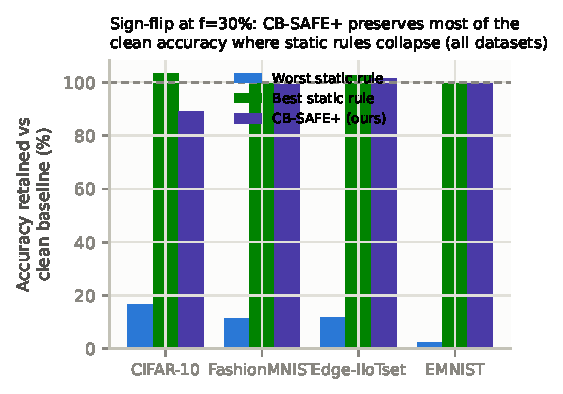
\includegraphics[width=\columnwidth]{fig_generalization.pdf}
\caption{Sign-flip at $f{=}30\%$: fraction of clean-baseline accuracy retained by
the worst static rule, the best static rule, and CB-SAFE+, on every dataset.
CB-SAFE+ preserves $84$--$97\%$ where static rules keep $12$--$60\%$.}
\label{fig:general}
\end{figure}

\subsection{The Privacy--Robustness Dial, Measured}
Fixing the rule (median) and sweeping cluster size traces the dial empirically
(Fig.~\ref{fig:cdial}). Without privacy ($c{=}1$), the median degrades gently from
50\% to 39\% as $f$ grows to $0.3$, i.e., classical robust aggregation. At $c{=}3$ the
same rule holds to $f{=}0.1$ (43.4\%) and collapses beyond; at $c{=}5$ degradation
begins already at $f{=}0.1$ (33.7\%): the breakdown frontier shifts left exactly as
$(1-f)^c$ predicts (Fig.~\ref{fig:tradeoff}). Two further observations sharpen the
picture. First, at $f{=}0.05$ privacy is \emph{free}: $c{=}3$ and $c{=}5$ match or
slightly exceed $c{=}1$ (52.2\% vs.\ 50.2\%), because cluster averaging denoises
before the median. Second, the dial's cost is refundable: at $c{=}3$, $f{=}0.3$,
where the private median collapses to 10\% against 39--41\% without privacy,
CB-SAFE+ recovers comparable accuracy \emph{while keeping the anonymity set},
by paying in rounds (warmup) rather than in privacy.

\begin{figure}[t]
\centering
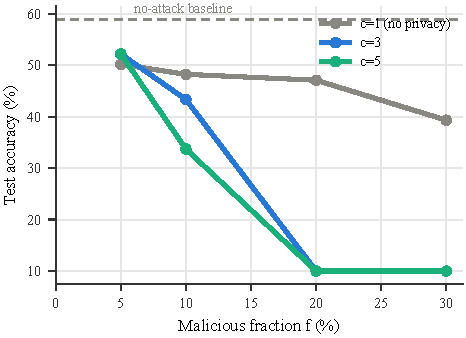
\includegraphics[width=\columnwidth]{fig_cdial.pdf}
\caption{The privacy--robustness dial, measured: median-rule accuracy under
sign-flip for $c\in\{1,3,5\}$. Larger anonymity sets shift the breakdown frontier
left, as $(1-f)^c$ predicts; at $f{=}5\%$ privacy costs nothing.}
\label{fig:cdial}
\end{figure}

\begin{figure}[t]
\centering
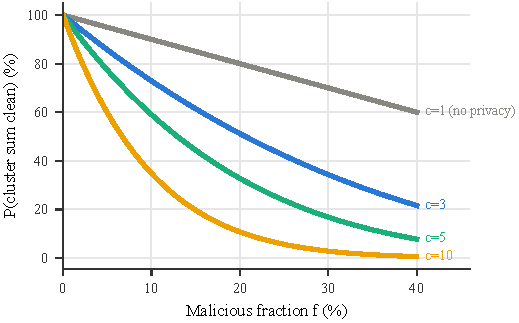
\includegraphics[width=\columnwidth]{fig_tradeoff.pdf}
\caption{The privacy--robustness dial, analytically: the anonymity set grows with
cluster size $c$, while the probability that a cluster sum is uncontaminated decays
as $(1-f)^c$.}
\label{fig:tradeoff}
\end{figure}

\section{Security Discussion and Limitations}
\textbf{What the design guarantees.} Within a cluster, privacy reduces to the
double-masking argument of \cite{bonawitz2017} with the DH-style key agreement
replaced by an IND-CCA2 KEM: masks are ChaCha20 outputs keyed by HKDF of
encapsulated secrets, so an honest-but-curious server colluding with fewer than $t$
cluster members learns only cluster sums. The robust layer never inspects anything
finer than a cluster mean. \textbf{What it does not.} We do not claim security
against an actively malicious server (who could misreport dropouts; standard
mitigations apply), nor differential privacy on the cluster sums themselves; the
anonymity set is bounded by the alive cluster size, and cluster sums of very small
clusters leak more than full-cohort sums. Robustness degrades predictably as
$k(1-f)^c$ approaches the trim capacity: at $c{=}3$, $f{=}0.3$ leaves an expected
$3.4$ clean clusters of 10, near the breakdown of a 2-per-side trimmed mean; this
is the price of the anonymity set and we report it rather than hide it. HQC
operations are $\sim$200$\times$ slower than ML-KEM's, which is immaterial here
(setup-only) but would matter for protocols that encapsulate per round.

\section{Conclusion}
CB-SAFE positions cryptographic diversity as a configuration choice rather than a
research programme: the KEM sits behind one interface, and the measured cost of
choosing the code-based occupant is a one-time setup constant. The more consequential
finding is what secure aggregation does to robustness: cluster averaging does not
merely dilute poisoning, it \emph{launders} it, transforming conspicuous attacks
into plausible-looking sums that defeat exactly the rules practitioners would reach
for. Defending therefore requires signals that survive aggregation (direction,
loss) accumulated over time. CB-SAFE+ shows one such design that identifies
individual attackers from group observations without spending any privacy. The open
questions our results make concrete: targeted backdoors remain invisible to
sum-level probes at every malicious fraction we tested, an actively malicious server
is outside our threat model, and the temporal identification argument should extend
to an adaptive attacker who modulates its poisoning to stay below the probe margin;
quantifying that game is the natural next step. Multi-seed replication and a
second dataset are in progress; the implementation and all measurement scripts are
released open-source as, to our knowledge, the first code-based reference point for
post-quantum secure aggregation in FL.

\begin{thebibliography}{9}
\bibitem{bonawitz2017} K.\ Bonawitz \emph{et al.}, ``Practical secure aggregation
for privacy-preserving machine learning,'' in \emph{Proc.\ ACM CCS}, 2017,
pp.\ 1175--1191.
\bibitem{nistir8545} National Institute of Standards and Technology, ``Status report
on the fourth round of the NIST post-quantum cryptography standardization process,''
NIST IR 8545, Mar.\ 2025.
\bibitem{fips203} National Institute of Standards and Technology,
``Module-lattice-based key-encapsulation mechanism standard,'' FIPS 203, Aug.\ 2024.
\bibitem{pqsf2024} X.\ Zhang, H.\ Deng, R.\ Wu, J.\ Ren, and Y.\ Ren, ``PQSF:
Post-quantum secure privacy-preserving federated learning,'' \emph{Sci.\ Rep.},
vol.\ 14, Art.\ no.\ 23553, 2024.
\bibitem{qinxu2025} X.\ Qin and R.\ Xu, ``Efficient post-quantum cross-silo
federated learning based on key homomorphic pseudo-random function,''
\emph{Mathematics}, vol.\ 13, no.\ 9, Art.\ no.\ 1404, 2025.
\bibitem{narsimhulu2026} P.\ Narsimhulu, P.\ Chithaluru, and R.\ Aluvalu,
``Efficient post-quantum cryptographic signature aggregation for low-latency
distributed networks,'' \emph{EURASIP J.\ Inf.\ Secur.}, vol.\ 2026, Art.\ no.\ 6, 2026.
\bibitem{byzpqfl2026} ``Byzantine-robust federated learning framework with
post-quantum secure aggregation for real-time threat intelligence sharing in
critical IoT infrastructure,'' arXiv:2601.01053, 2026.
\bibitem{cqsa2026} ``CQSA: Byzantine-robust clustered quantum secure aggregation in
federated learning,'' arXiv:2602.22269, 2026.
\bibitem{singh2025pqfog} J.\ Singh, P.\ Singh, A.\ Kaur, and M.\ Hedabou,
``Post-quantum secure fog-edge computing using federated learning with blockchain,''
\emph{J.\ Supercomput.}, vol.\ 81, Art.\ no.\ 1249, 2025.
\bibitem{fltrust} X.\ Cao, M.\ Fang, J.\ Liu, and N.\ Z.\ Gong, ``FLTrust:
Byzantine-robust federated learning via trust bootstrapping,'' in \emph{Proc.\ NDSS},
2021.
\bibitem{zeno} C.\ Xie, S.\ Koyejo, and I.\ Gupta, ``Zeno: Distributed stochastic
gradient descent with suspicion-based fault-tolerance,'' in \emph{Proc.\ ICML}, 2019.
\bibitem{bell2020} J.\ H.\ Bell, K.\ A.\ Bonawitz, A.\ Gasc\'on, T.\ Lepoint, and
M.\ Raykova, ``Secure single-server aggregation with (poly)logarithmic overhead,''
in \emph{Proc.\ ACM CCS}, 2020, pp.\ 1253--1269.
\bibitem{blanchard2017} P.\ Blanchard, E.\ M.\ El Mhamdi, R.\ Guerraoui, and
J.\ Stainer, ``Machine learning with adversaries: Byzantine tolerant gradient
descent,'' in \emph{Proc.\ NeurIPS}, 2017, pp.\ 119--129.
\bibitem{yin2018} D.\ Yin, Y.\ Chen, R.\ Kannan, and P.\ Bartlett,
``Byzantine-robust distributed learning: Towards optimal statistical rates,'' in
\emph{Proc.\ ICML}, 2018, pp.\ 5650--5659.
\bibitem{bagdasaryan2020} E.\ Bagdasaryan, A.\ Veit, Y.\ Hua, D.\ Estrin, and
V.\ Shmatikov, ``How to backdoor federated learning,'' in \emph{Proc.\ AISTATS},
2020, pp.\ 2938--2948.
\bibitem{brea2021} J.\ So, B.\ G\"uler, and A.\ S.\ Avestimehr,
``Byzantine-resilient secure federated learning,'' \emph{IEEE J.\ Sel.\ Areas
Commun.}, vol.\ 39, no.\ 7, pp.\ 2168--2181, 2021.
\bibitem{nguyen2025lattice} H.\ Nguyen, S.\ Huda, Y.\ Nogami, and T.\ T.\ Nguyen,
``Security in post-quantum era: A comprehensive survey on lattice-based
algorithms,'' \emph{IEEE Access}, vol.\ 13, pp.\ 89003--89024, 2025.
\end{thebibliography}

\end{document}
